\lesson{17 Seq 2024}{Basics}

Linux treats everything as a file.

\begin{definition}[Program]
A program is an executable file.
\end{definition}

\begin{definition}[Process]
A process is a program instance.
\end{definition}

A program comes with an ID, an address space (text, data, heap, and stack segments\footnote{There are more segments, e.g., BSS, in actual implementation.}), execution context (processor registers), files, signals, and threads.

\begin{note}
A process is the granularity of \textbf{protection}.
\end{note}

\begin{definition}[Thread]
A thread is an execution context.
\end{definition}

A thread comes with an ID, registers (PC and SP), and stack. All threads share a process's address space. Threads can exploit multiprocessors and enable concurrency and parallelism.

There are 2 sorts of threads:

\begin{enumerate}
    \item kernel thread
    \item user-level thread
\end{enumerate}

Kernel threads are managed \textcolor{gray}{and scheduled} by OS. They are manipulated via syscalls. The thread table lives in OS kernel. Whereas user-level threads are managed by a user space library. Per-process thread table lives in the process address space, such that the user space scheduler is fully aware of what an application demands.

\begin{note}
User-level threads are at least an order of magnitude faster than kernel threads.
\end{note}

User-level threads exploit concurrency with different \textit{threading modeling}. There are 1:1, N:1, and M:N models.

\subsection{Linux process management}

Below is state transition diagram of Linux process management\footnote{The diagram captures primary states for illustrative purpose; there are more states in actual implementation.}.

\begin{figure}[H]
\centering
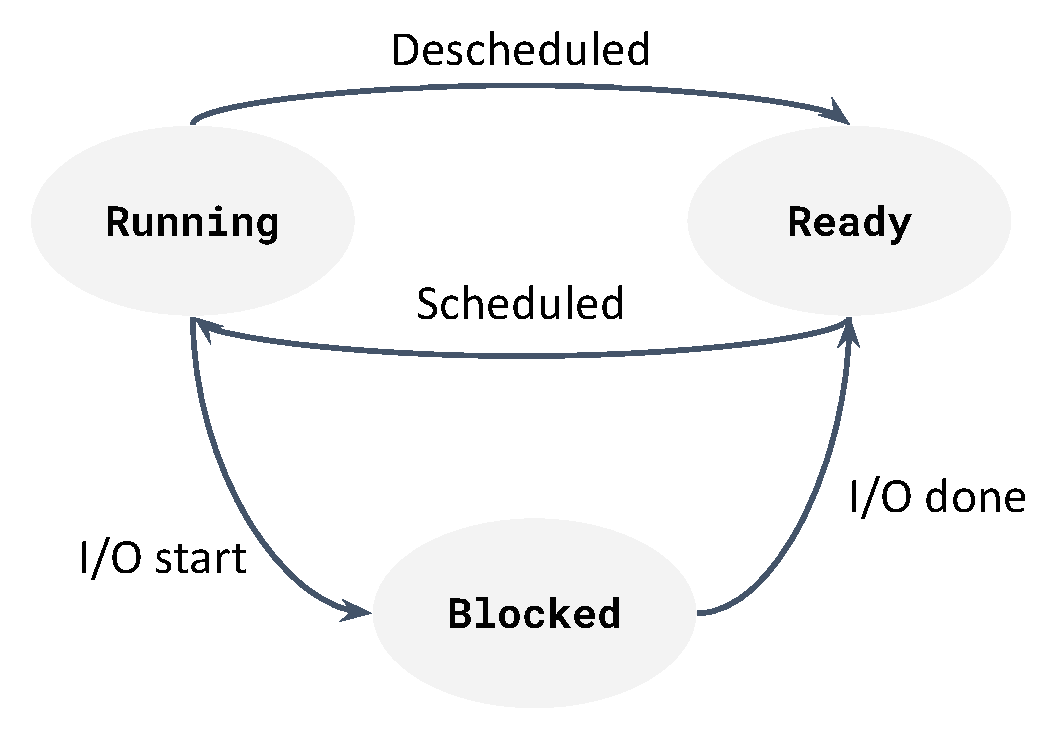
\includegraphics[width=0.5\linewidth]{figures/transition.eps}
\end{figure}

The figure below illustrates some of Linux process-related syscalls.

\begin{figure}[H]
\centering
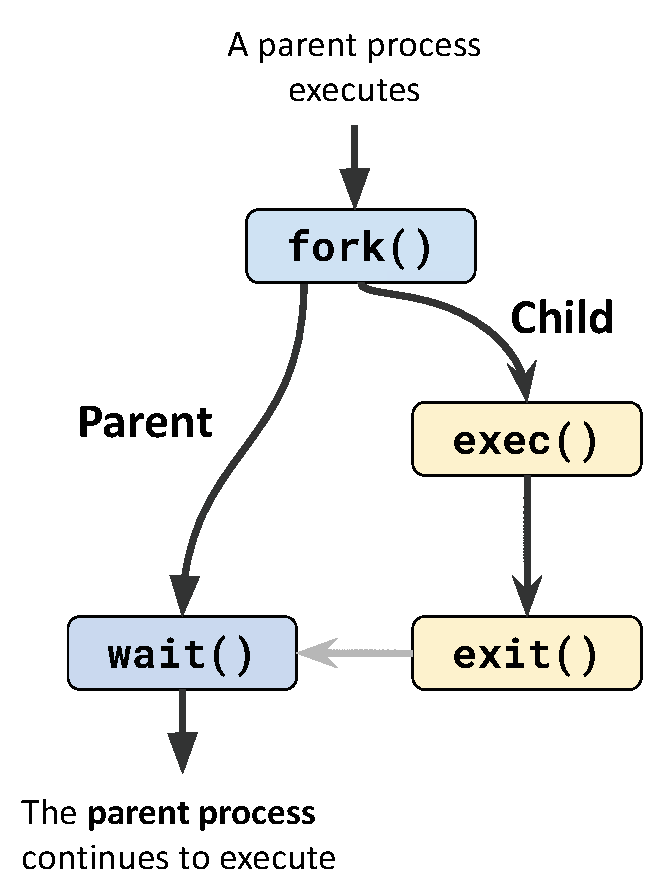
\includegraphics[width=0.35\linewidth]{figures/lifetime.eps}
\end{figure}

\verb|fork| creates a new process by copying its parent\footnote{Such operation is copy-on-write (COW). All states including the entire address space, file descriptors, etc. are copied.}. Both the parent and the child run the same program from the same ``line" after \verb|fork|. \\

To force the child process to run something else, use the \verb|exec| syscall. Address space are replaced, but file descriptors such as \verb|stdin|, \verb|stdout|, and \verb|stderr| are preserved.

\begin{note}
\verb|fork| and \verb|exec| enable initiating a different process within a process, rather than OS kernel, in a divide-and-conquer fashion. \\

Use cases of such a combination are redirecting I/O, to switch users, and to switch working directory.
\end{note}

\verb|exit| terminates a process. The process is now in ``zombie" state; it can be ``reaped" by its parent process via the \verb|wait| syscall. \verb|wait| suspends a process until \textbf{one of}\footnote{Use a loop to wait for all child processes} its child process transitions state. Linux \verb|init| process reaps all other processes.

Linux \textit{thread group} is a set or threads of the same process. Each thread group comes with a single leader, usually the first thread in the group. A thread group is a granularity for ``task" management to receive signals. When all members of a group terminate, a single \verb|SIGCHILD| signal is sent to the parent process\footnote{In this sense, a thread group is also a granularity to send signals.}.

On \verb|exec|, all threads but the leader in a thread group terminate, whereas the group leader executes the ``new" program.

\begin{note}
Linux does not distinguish a process from a \textcolor{kernel}{thread}. They both share \verb|task_struct|, which takes over 3.5 KB memory\footnote{This is the reason for expensive syscall \verb|fork.}
\end{note}

Similar to \verb|fork|, the \verb|clone| syscall also creates a process. There are 2 major differences:

\begin{enumerate}
    \item \verb|clone| can also creates a thread;
    \item \verb|clone| allows fine-grained control over execution state to share \textcolor{gray}{with the new ``task"} via the \verb|flags| argument
\end{enumerate}

Linux kernel threads do \textbf{not} have their own address space and run entirely in kernel space. They are all ``forked" from \verb|kthreadd|.
